\documentclass{article}

\usepackage[%
    left=0.5in,%
    right=0.5in,%
    top=0.5in,%
    bottom=0.5in,%
]{geometry}%
\usepackage{minitoc}
\usepackage{multicol}
\usepackage{graphicx}
\usepackage{fixltx2e}
\usepackage{listings}
\usepackage{color}
\usepackage{caption,setspace}
\usepackage{hyperref}
    \hypersetup{ colorlinks = true, linkcolor = blue }
\usepackage{blindtext}
\definecolor{lightgray}{gray}{0.9}
\graphicspath{ {./} }

\newcommand{\inlinecode}[2]{\colorbox{lightgray}{\lstinline
[language=#1]$#2$}}
\newcommand{\worddef}[1]{\hyperref[sec:reference]{\textit{#1}}}
\captionsetup{width=0.8\linewidth}

\begin{document}

\tableofcontents

\newpage

\section{Limitations of simple reactive architecture}
no representation of the environment means
\begin{itemize}
  \item its knowledge of the world is limited by the \textbf{range of its sensors }
  \item it’s unable to count (as opposed to recognise number)
  \item it’s unable to recover from actions which fail silently – and many others
\end{itemize}

\begin{multicols}{2}

\section{Modelling reactive behaviours}
\begin{center}
  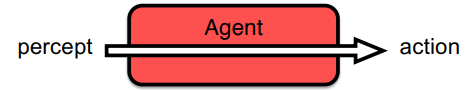
\includegraphics[scale=0.5]{reactive_agent.png}
\end{center}

\begin{itemize}
  \item we can model reactive behaviours as condition-action rules 
  \item if the condition matches the agent’s precepts, it triggers an action \texttt{if percept then action }
  \item a simple reactive agent maintains no internal representation of the state of the world, whether the rule has been fired before etc.
\end{itemize}


\section{Reactive architectures with state}

\begin{center}
  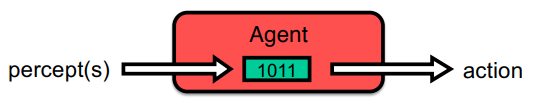
\includegraphics[scale=0.5]{reactive_state_agent.png}
\end{center}

\begin{itemize}
  \item some rules match against an internal representation of aspects of the environment 
  \item representations can be built using simple \textbf{percept-driven rules} (internal actions) which record simple ‘beliefs’ about the state of the world
\end{itemize}

\end{multicols}

\section{State}

\begin{itemize}
  \item we have simply taken a condition-action rule which matched against a percept and generated an action and split it in two, with a mediating internal representation 
  \item needs extra machinery to store the state 
  \item requires at least \textbf{two computation steps} to choose an action rather than one
\end{itemize}

\subsection{Actions which modify the internal state}

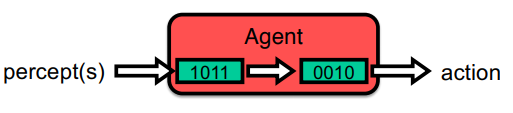
\includegraphics[scale=0.5]{reactive_state_agent_modify.png}

\begin{itemize}
  \item we can extend this to rules
  \begin{itemize}
    \item whose conditions match against the agent’s internal state; and
    \item whose actions modify the agent’s internal state 
  \end{itemize}
  \item again, this appears to make things worse: requires even \textbf{more space and more steps} to choose an action
\end{itemize}

\subsection{Importance of representations}
\begin{itemize}
  \item notion of a rule which only responds to and generates internal changes in the agent is a key step 
  \item forms the basis of all derived representations, and of representations which refer to other aspects of the agent’s internal state 
  \item e.g., allows the agent to respond only to changes in the environment, ignoring features that are constant 
  \item without some representation of the previous state, we can’t say what is novel in the current state
\end{itemize}

\section{Detecting change}

\begin{center}
  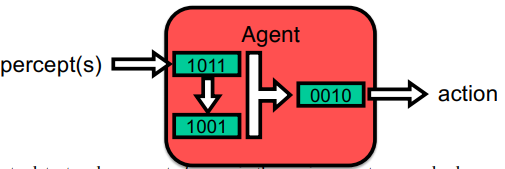
\includegraphics[scale=0.5]{agent_change.png}
\end{center}

\begin{flushleft}
to detect and represent changes in the environment we need rules
\begin{itemize}
  \item whose conditions match against representations of the current and previous precepts 
  \item whose action is to remember (copy) the state representing the current percept for use at the next cycle
\end{itemize}
\end{flushleft}

\subsection{Internal representations}
\begin{itemize}
  \item require more space and incur the cost of maintaining the representation 
  \item allow the choice of actions based on sequences of states, e.g.: to react to change or \textbf{lack of it}
  \item given such internal behaviours, much more complex external behaviours are possible
\end{itemize}

\section{Action selection function}
\begin{itemize}
  \item the action selection function for a reactive agent with state looks like 
  \begin{itemize}
    \item $selectAction : (Event, State) \rightarrow (Action, State)$
  \end{itemize}
  \item a reactive agent with state (finite-state machine) can respond to regular sequences of events 
  \item we can add more complex state data structures to increase the capabilities of the agent, e.g.,
  \begin{itemize}
    \item add a stack (pushdown automata) to respond to context-free sequences 
    \item add a random-access array to get a Turing machine, etc.
  \end{itemize}
\end{itemize}

\section{Advantages of state}
\begin{itemize}
  \item agent’s knowledge of the world is \textbf{no longer limited} by the range of its sensors, it can remember parts of the environment it can’t currently sense 
  \item agent is \textbf{able to count}, allowing it to execute behaviours that require some action to be \textbf{iterated} a given number of times 
  \item agent is able to \textbf{recover} from actions which \textbf{fail silently}, it can remember which actions it has tried before or how many times an action has been tried, and \textbf{try something else} if the action doesn’t have the desired effect
\end{itemize}

\subsection{Combined actions}
\begin{center}
  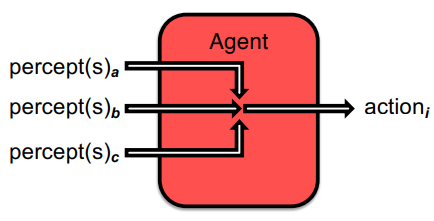
\includegraphics[scale=0.5]{combined_actions.png}
\end{center}
\begin{center}
  distinct actions triggered by different percepts are combined into a \textbf{single composite action}
\end{center}

\subsection{Problems with combining actions}
\begin{itemize}
  \item action selection based on combining actions is \textbf{prone to a number of problems}:
  \begin{itemize}
    \item \textbf{local minima}: e.g., Braitenberg vehicles get suck between to obstacles, unable to turn around
    \item \textbf{cyclic behaviour}: e.g., Braitenberg vehicles get trapped orbiting an obstacle 
  \end{itemize}
  \item one way to solve these problems is simply to inject \textit{noise} or \textit{randomness} into the agent’s behaviours
\end{itemize}

\subsection{Cyclic behaviour}
\begin{flushleft}
Occurs when an agent repeats it's actions creating an infinite loop.
\end{flushleft}

\subsection{Local minima}
\begin{flushleft}
consider a simple ‘boids-like’ agent which chooses an action by combining 
\begin{itemize}
  \item a vector towards the goal 
  \item a vector away from an obstacle (if any)
\end{itemize}
if there is an obstacle on the way to the goal, the agent can get stuck. Image a scenario where the goal is straight line from the agent and there is a single obsticle in front of it. One vector would try to move towards the goal, where the other would push against the obsticle. Both of them cancel each other out, leaving the agent stuck in a single place.
\end{flushleft}

\subsection{Escaping local minima with random vector}
\begin{itemize}
  \item adding a (small) random vector can take the agent past the obstacle, "unsticking" it. It would allow for the machine to move slightly while two initial vectors cancel each other out.
  \item However this would not work if the obsticle surounds the agent.
\end{itemize}

\subsection{Avoid Past behaviour}
\begin{itemize}
  \item Avoid Past behaviour uses a short term representation of where the agent has been recently \textbf{stored in memory}
  \item repulsive forces are generated from recently visited areas 
  \item the output of the Avoid Past behaviour is a vector of the same form as the vectors produced by the other behaviours (e.g., move to goal, avoid obstacles etc.) and is combined in the same way 
  \item memory used by Avoid Past is \textbf{short term}. The agent \textbf{can return} to previously visited locations when the memory decays
\end{itemize}
\begin{center}
  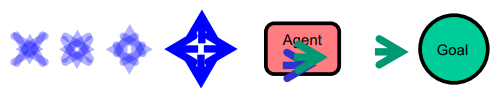
\includegraphics[scale=0.5]{avoid_past.png}
\end{center}
\begin{flushleft}
This however still have a problem. The memory is short term, meaning that nothing prevents the agent from repeating the same mistake after a while. It could get stuck in \textit{cycling behaviour}
\end{flushleft}

\subsection{Subsumption architecture}

\begin{itemize}
  \item \textbf{collection of behaviours} specified as a set of rules in Behavior Language 
  \item behaviours compile to an Augmented Finite State Machine (AFSM) 
  \item each AFSM performs an action and is responsible \textbf{for its own perception of the world}
  \item the output of one behaviour can \textbf{form the input to another}
\end{itemize}

\begin{center}
\begin{minipage}{0.48\linewidth}
  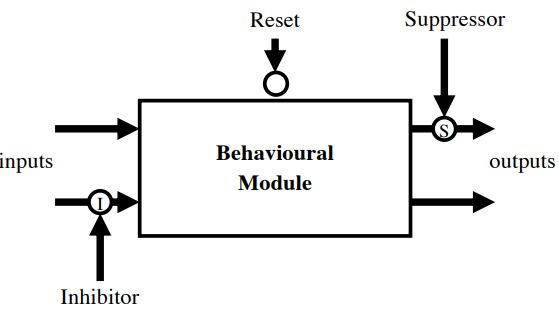
\includegraphics[scale=0.5]{behaviour_model.png}
\captionof{figure}{Behavioural model}
\end{minipage}%
\end{center}

\begin{itemize}
  \item behaviours are organised into layers, each of which is responsible for \textbf{independently achieving a goal}
  \item complex actions subsume simpler behaviours lower in the hierarchy 
  \item output of lower layers \textbf{can be read by higher layers }
  \item lower layers have \textbf{no knowledge} of higher layers 
  \item layers operate \textbf{concurrently and asynchronously}
  \item higher layers control lower ones using:
  \begin{itemize}
    \item \textbf{inhibition}: prevents transmission 
    \item \textbf{suppression}: replaces a message with a suppressing message
    \item \textbf{reset}: restores behaviour to its original stat
  \end{itemize}
\end{itemize}

\subsection{Foraging}
\begin{itemize}
  \item behaviours are prioritised and the robot is executing only \textbf{one behaviour at any one time} 
  \item when the robot senses an obstacle, \textbf{wandering is suppressed}, so that the avoidance behaviour can get the robot away from the obstacle 
  \item when the robot senses the target object, \textbf{collision avoidance is suppressed}, otherwise the pickup behaviour couldn’t get the robot close enough to the object to pick it up 
  \item when the object is grabbed, homing then \textbf{suppresses pickup} (allowing the robot to ignore the potential distraction of of other objects it might encounter on its way back to base)
\end{itemize}

\section{Advantages of stateful reactive architecture}
\begin{itemize}
  \item a reactive architecture with state can \textbf{produce any kind of behaviour} (no longer restricted to a fixed response to a given situation) 
  \item no complex problem solving required 
  \item if the state can be partitioned (e.g., subsumption architecture)
  \begin{itemize}
    \item development is easier 
    \item can still use dedicated, parallel hardware
    \item fast (real-time) response to changes in the environment
  \end{itemize}
\end{itemize}

\section{Disadvantages of stateful reactive architectures}
\begin{itemize}
  \item all responses must be defined in advance 
  \item can’t cope with novel situations for which they don’t have a predefined behaviour 
  \item agent programs for complex problems can be very large
\end{itemize}

\pagebreak
\section*{Reference section} \label{sec:reference}
\begin{description}
	\item[placeholder] \hfill \\
\end{description}
\end{document}
